\chapter{Mixed Reality for Human-Robot Collaboration}%
\label{chapter:on-site}
% \chapter{On-site Member's Application}% first title of section

After having properly implemented the bidirectional communication between both environments, the on-site and the remote, allowing both members to interact with the robot, the next step was to complement the already built application as well as its interface. 

\section{On-site Application Features}
\label{section:on-site-features}
% \input{chapters/on-site/on-site-features} commented this part because text is below - choose whether to use this or the text below
Regarding the on-site member's collaboration experience, as explained in the state of art review, by implementing different sensorial cues, such as visual and audio, it will enhance the user experience into a more intuitive and immersive way.
    
    \subsection{Virtual Safety Zones}
    \label{subsection:virtual-safety-zones} 
    % \input{chapters/on-site/subsections/virtual-safety-zones} commented this part because text is below - choose whether to use this or the text below

        The implementation of virtual safety zones is a critical feature designed to enhance on-site member's safety when interacting with the robot. 

        Two safety zones were developed, as shown in figure \ref{fig:dual-safety}, to address specific safety and user experience concerns:

        \begin{itemize}
            \item \textbf{Outer Safety Zone}: Initially, only the outer safety zone was developed. The purpose of creating this zone was to provide an 
            early warning to users as they approach the hazardous area near the robot. This approach consisted on changing its color as a visual alert. 
            However, this method proved ineffective because, once inside it, users could not perceive the color change, rendering the warning system inadequate.
            
            \item \textbf{Inner Safety Zone}: To overcome the limitations of the outer zone, an additional, inner safety zone was introduced. 
            This design ensures a two-step safety mechanism:

                \textbf{Visual Alert}: Upon entering the outer safety zone, the color of the inner sphere changes to red. 
                This alteration serves as a visual cue, indicating that the user is getting closer to a high-risk area.

                \textbf{Auditory Warning}: Entering the inner safety zone triggers an auditory alarm. This sound alert signifies that the user has 
                breached into the robot working area, enhancing the effectiveness of the safety mechanism.
        \end{itemize}

        \begin{figure}[h]
            \centering
            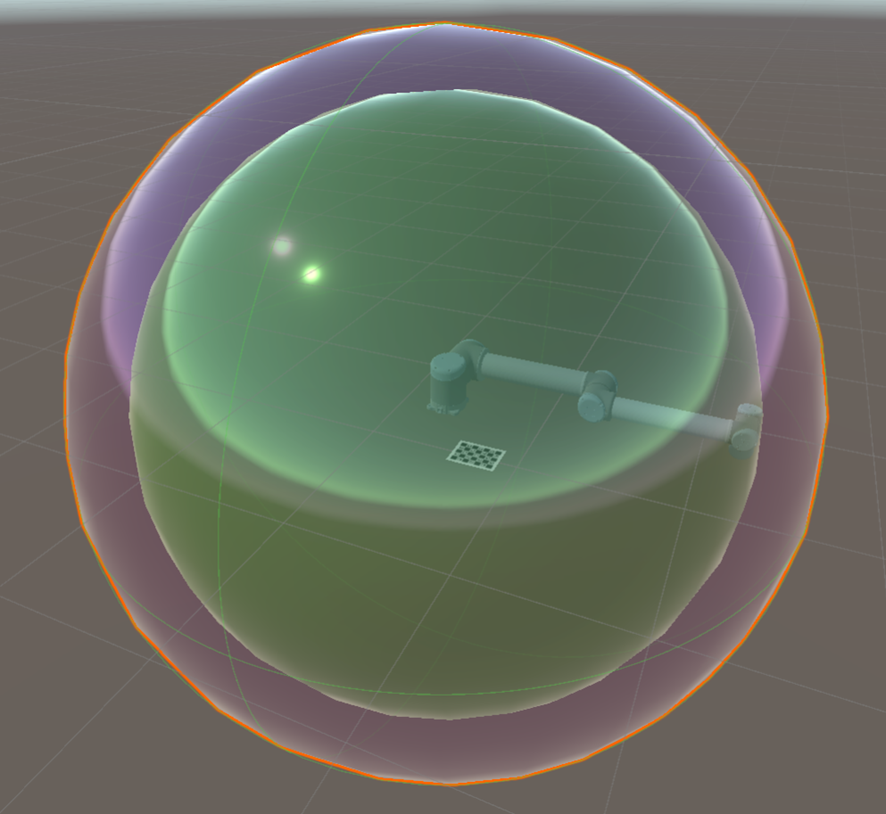
\includegraphics[width=0.5\linewidth]{figs/dual-safetyzone-robot.png}
            \caption{Simulated environment showing the display of both the inner and outer safety zones, as well as the robot and the marker inside them}
            \label{fig:dual-safety}
        \end{figure}

        \subsubsection{Safety Zone Breach Protocol}

            A crucial safety feature is that if the on-site member enters the safety zone area while the robot is in motion, the robot 
            automatically stops. This immediate halt ensures that potential accidents or injuries are avoided by preventing any interaction 
            with the robot when a user is within a designated dangerous area.
                
    \subsection{Interface}

        The interface, which incorporates the safety-zone features detailed earlier, is illustrated in figure \ref{} (take another picture with the most recent interface) 
        Within this interface, one can observe the panel for controlling the robot joints. Additionally, there are two green buttons 
        positioned at the top and bottom right corners of the interface, designated for activating the safety-zone and joint movement functions, 
        respectively. This subsequent features will be explained below.

        \begin{figure}[h]
            \centering
            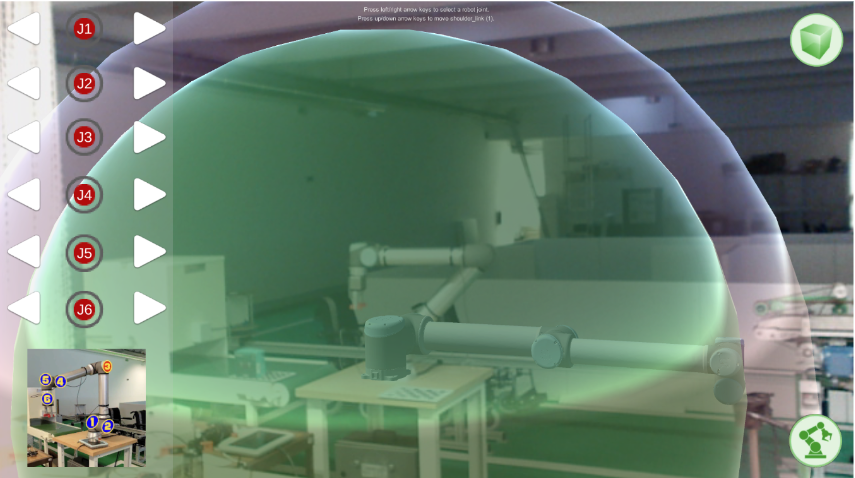
\includegraphics[width=1\linewidth]{figs/interface.png}
            \caption{Interface featuring developed interactions}
            \label{fig: interface}
        \end{figure}

        \subsubsection{Joint Movement} - this is explained also in the previous chapter (3) - includes a pseudo-code snippet

            This feature allows users to manipulate the robot's joints via a user-friendly interface, as depicted in the figure \ref{fig:joint-1} 
            by the first joint. Its functionality works as follows:


            \begin{itemize}
                \item \textbf{Joint Selection}: Users can activate a joint by clicking on it. Upon activation, the 
                selected joint's central red circle turns green.
                \item \textbf{Movement Control}: By clicking on the selected joint's directional arrows within the interface, it moves in either a 
                positive or negative direction. This functionality mimics the real-time movement control similar to using keyboard arrow keys, ensuring 
                intuitive operation.
                \item \textbf{Continuous Movement}: The selected joint continues to move until we deactivate its button.
                \item \textbf{Single Joint Activation}: To ensure precise control, joint movement is only possible when one joint is selected at a time. 
                This prevents unintended actions and enhances the accuracy of adjustments.
            \end{itemize}
        
        
        \subsubsection{Buttons}
        
            Two buttons, shown in figure \ref{fig:joint-toggle}, were introduced to toggle the activation and deactivation of the joint menu 
            functionalities \ref{fig:toggle-joint} and the safety zones \ref{fig:toggle-safety}. Upon deactivation, the button will turn gray. 
            This design allows users to easily switch these features on or off, providing flexibility in controlling the safety mechanisms and movement 
            operations within the \ac{XR} environment.
            
            
            \begin{figure}[h]
            \centering
            \begin{subfigure}[b]{0.31\textwidth}    
                \centering
                
\includegraphics[width=1\linewidth]{figs/joint-1.png}
                \caption{Joint Control for first Joint}
                \label{fig:joint-1}
                \end{subfigure}
            \hfill % This command adds space between the subfigures
            \begin{subfigure}[b]{0.31\textwidth}
                \centering
                
\includegraphics[width=0.3\linewidth]{figs/clicked_joints.png}
                \caption{Controller Menu Toggle}
                \label{fig:toggle-joint}
            \end{subfigure}
            \hfill
            \begin{subfigure}[b]{0.31\textwidth}
                \centering
                
\includegraphics[width=0.3\linewidth]{figs/unclick_sz.png}
                \caption{Safety-zone Toggle}
                \label{fig:toggle-safety}
            \end{subfigure}
            \caption{Example from first joint control menu and toggle buttons for controller menu and safety-zones}
            \label{fig:joint-toggle}
            \end{figure}
        
% \section{Video Demo}
%     The video demonstration (\href{https://www.youtube.com/watch?v=SMQ0yXhdnUo}{https://www.youtube.com/watch?v=SMQ0yXhdnUo}) showcases 
%     the successful implementation of the previously described features. Testing of the application was conducted using a laptop paired
%      with the camera depicted in the figure \ref{fig:camera-c922}. This approach was chosen due to encountered challenges in properly
%       building the application for android \ac{HHD}.
            

% previously was a chapter - re-define its order in the document
\section{Remote Collaboration}
% \label{chapter:remote}
% \begin{introduction}
% The development of the remote member's application will be thoroughly explained in this chapter.
% \end{introduction}

    After having successfully implemented the robot's digital model into the Unity environment, as well as performed the pose registration, 



    Building on the foundation of the application that facilitated on-site member interactions, the next critical step was to establish a robust connection to the UR10e robot. This connection was essential for accurately developing a digital twin of the robotic arm, allowing for real-time manipulation and visualization within a Unity environment.

    To achieve this, it was necessary to extend the initial project by developing a complementary application focused on the remote manipulation 
    of the robotic arm through Unity. 

    This bridge facilitated communication between the ROS environment on Ubuntu and the Unity application on Windows, enabling real-time visualization 
    and control of the robot within Unity.

    However, this integration posed significant challenges. Despite the potential of the ROS-TCP-Connector, the documentation provided limited guidance 
    on adapting the connection to different robots beyond the examples in the online tutorial. As a result, the development process relied heavily on 
    trial and error, requiring iterative testing and debugging to achieve a functional ROS-Unity connection.

    
    
    
    \section{New Control Types for Remote Operation}
    To maintain previously developed code and introduce necessary functionalities for remote operation, three distinct control types were implemented in the \texttt{Controller.cs} script, responsible for controlling the digital twin version of the robot:
    
    \begin{enumerate}
        \item \textbf{UIButtonControl:} Originally developed for the on-site member application, this control type features a UI interface with safety-zone functionalities. It allows operators to interact safely and efficiently with the robot. Its implementation was detailed in the previous chapter.
        \item \textbf{Position Control:} This control type enables the manual control of the robot's joints through direct user input. It captures and sends the Unity digital twin's joint positions to the ROS environment upon user command, facilitating precise adjustments and real-time interaction.
        \item \textbf{Joint State Subscription:} This control type continuously updates the Unity digital twin based on joint state data received from ROS. It ensures the digital twin accurately reflects the physical robot's status, automating synchronization between the Unity model and the ROS data.
    \end{enumerate}
    
    %%%%%%%%%%%%%%%%%%%%%%%%%%%%%%%%%%%%%%%%%%%%%%%%%%%%% good for introducing the control types when explaining them (jointControl and JointStateSub) - remove after having both control types well documented
    % \subsubsection{Practical Implementation of Control Types}
    % The \texttt{Controller.cs} script was enhanced to facilitate various operational modes:
    % \begin{itemize}
    %     \item \textbf{UI Button Control:} Offers a user-friendly interface that non-technical users can use to interact with the robot, simplifying the control mechanism and enhancing the user experience by utilizing pre-set safety zones and interactive controls.
    %     \item \textbf{Position Control:} Allows operators to manipulate the robot's joints in real-time via direct interaction, providing a highly interactive and responsive control environment.
    %     \item \textbf{Joint State Subscription:} Ensures that any changes in the robot's state in the ROS environment are immediately reflected in the Unity simulation, enhancing the accuracy of the digital twin.
    % \end{itemize}
    %%%%%%%%%%%%%%%%%%%%%%%%%%%%%%%%%%%%%%%%%%%%%%%%%%%%%
        
    
    \subsubsection{Integration Highlights}
    These two nodes addressed key aspects of system performance:
    \begin{itemize}
        \item \textbf{Synchronization:} Ensures that changes in Unity’s control environment are accurately and timely reflected in the robot's physical movements.
        \item \textbf{Modularity:} Separates data handling and robot control into different nodes to improve system reliability and ease of maintenance.
    \end{itemize}




    
    %%%%%%%%%%%%%%%%%%%%%%%%%%%%%%%%%%%%%%%%%%%%%%%%%%%%%%%%%
    do below here - add photos or video that mimic the process, same images
    
    \section{Camera Feed Transmission}

    In order to enhance the remote participant's understanding of the on-site environment and task performance, I integrated a live camera feed from a camera that was attached to the robot. This feed was then displayed in the Unity application, allowing the remote user to observe the robot's environment in real-time, providing critical visual feedback necessary for effective remote collaboration.

    \subsection{Hardware and Software Setup}
    An Orbbec Astra camera, displayed in the figure \ref{fig:astra-camera}, was provided by the project supervisors was used to capture the live video feed. This 3D camera was chosen for its high-quality video output and compatibility with the ROS environment, enabling seamless integration into the Unity application.
    
    \begin{figure}[h]
        \centering
        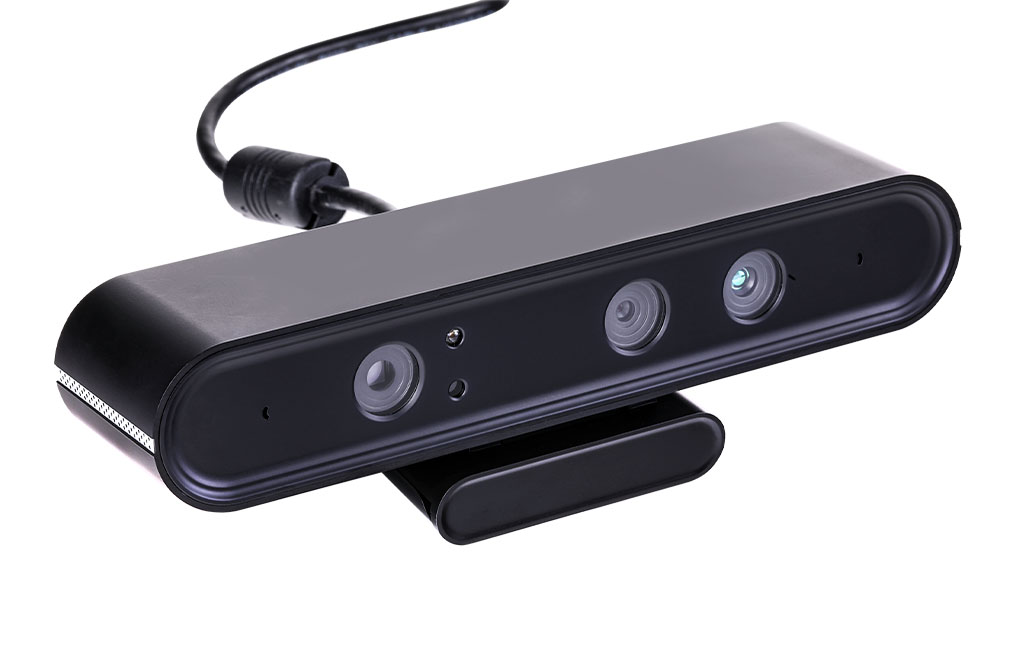
\includegraphics[width=0.7\textwidth]{figs/AstraSeries_3.jpg}
        \caption{Astra 3D Orbbec Camera used to transmit real-time video feed from robot environment to remote user}
        \label{fig:astra-camera}
    \end{figure}
    \FloatBarrier

    To integrate the camera into the ROS environment, an existing GitHub repository \footnote{Github Repository used to integrate Astra Orbbec Camera in the ROS environment \url{https://github.com/orbbec/ros_astra_camera} Accessed: 2024-10-04} tailored for the Astra camera integration was used. This repository contained the necessary drivers and ROS nodes to enable the camera's functionality within the ROS framework.

    \subsection{ROS Camera Node}
    To initiate the camera feed, the \texttt{astra\_camera\_node} from the \texttt{astra\_camera} package is initialized. Afterwards, an RVIZ image viewer was used to visualize the live feed, ensuring the camera was functioning correctly and capturing the desired video data.

    \subsection{Unity Camera Feed Integration}
    From the Unity side, the \texttt{CameraFeedReceiver.cs} (verify the name of the script) script was developed to receive and display the live camera feed. This script was then atached to an UI interface (confirm the name of the element) that displayed the video feed in real-time. 
    add a figure of the UI interface with the view of the camera - The figure \ref{fig:camera-feed} (add figure) illustrates the camera feed in the Unity application, showcasing the live video stream from the robot's environment.

    \subsection{Data Transmission to Unity} 
     
    However, the raw image data generated by the camera was too heavy to be transmitted efficiently over Wi-Fi, so this data needed to be republished using the \texttt{image\_transport} package.
    By utilizing the following \ac{ROS} command 
    \begin{verbatim}
        rosrun image_transport republish raw 
        in:=/camera/color/image_raw out:=/camera/image_repub
    \end{verbatim}
    the image data was republished in a more efficient format, allowing for smoother and real-time transmission to the Unity environment.
    

